\documentclass[border=10pt]{standalone}
\usepackage{amsmath}
\usepackage{pgfplots}
\usepgfplotslibrary{fillbetween}
\pgfplotsset{compat=1.16}
\begin{document}
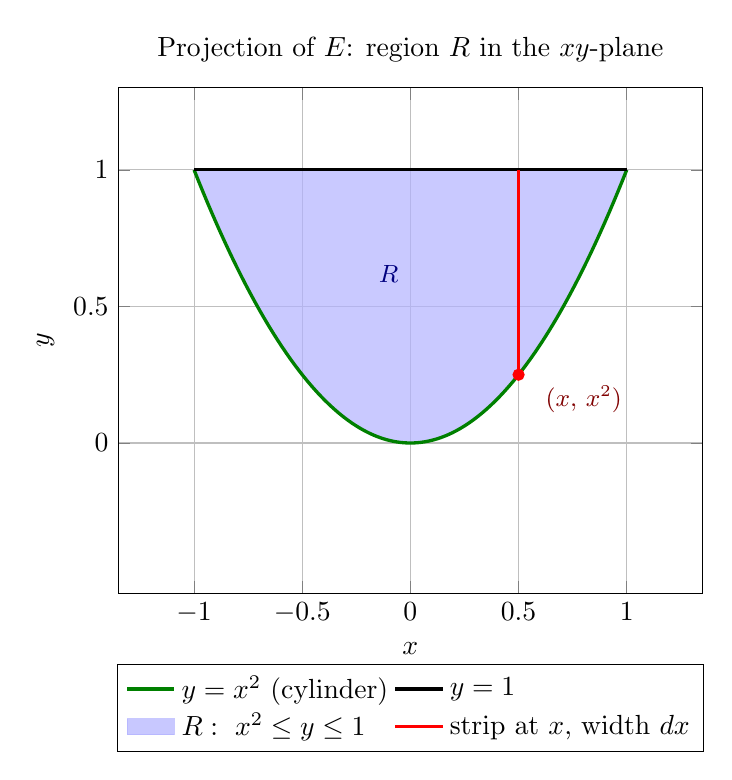
\begin{tikzpicture}
\begin{axis}[
    width=9cm, height=8cm,
    xlabel={$x$}, ylabel={$y$},
    xmin=-1.35, xmax=1.35, ymin=-0.55, ymax=1.3,
    xtick={-1,-0.5,0,0.5,1}, ytick={0,0.5,1},
    grid=major, title={Projection of $E$: region $R$ in the $xy$-plane},
    legend style={at={(0.5,-0.14)}, anchor=north, legend columns=2},
    legend cell align=left,
]
\addplot[name path=parab, green!50!black, very thick, domain=-1:1, samples=100] {x^2};
\addlegendentry{$y=x^2$ (cylinder)}
\addplot[name path=line, black, very thick, domain=-1:1, samples=2] {1};
\addlegendentry{$y=1$}
\addplot[blue!30, opacity=0.7] fill between[of=parab and line];
\addlegendentry{$R:\ x^2\leq y\leq 1$}
\addplot[red, very thick] coordinates {(0.5,0.25) (0.5,1)};
\addlegendentry{strip at $x$, width $dx$}
\addplot[only marks, mark=*, red] coordinates {(0.5,0.25)};
\node[anchor=west, text=red!50!black] at (axis cs:0.58,0.16) {\small $(x,\,x^2)$};
\node[anchor=south, text=blue!50!black] at (axis cs:-0.1,0.55) {\small $R$};
\end{axis}
\end{tikzpicture}
\end{document}
